107. Возможны два случая расположения данных углов: оба внутри образующегося при пересечении треугольника, или один угол внутри, а другой --- снаружи. В первом случае картинка имеет следующий вид:
\begin{figure}[ht!]
\center{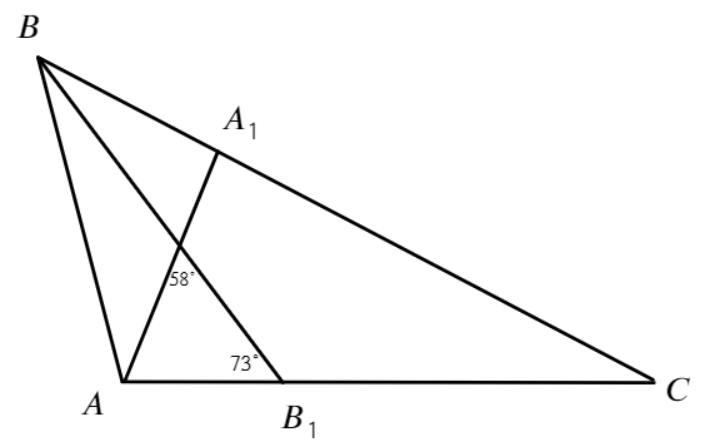
\includegraphics[scale=0.35]{g107.png}}
\end{figure}\\
Найдём $\angle A_1AC=180^\circ-58^\circ-73^\circ=49^\circ,$ значит $\angle A=2\cdot49^\circ=98^\circ.$ Тогда $\angle ABB_1=180^\circ-98^\circ-73^\circ=9^\circ,\ \angle B=2\cdot9^\circ=18^\circ,\ \angle C=180^\circ-98^\circ-18^\circ=64^\circ.$\\
Во втором случае картинка имеет следующий вид:
\begin{figure}[ht!]
\center{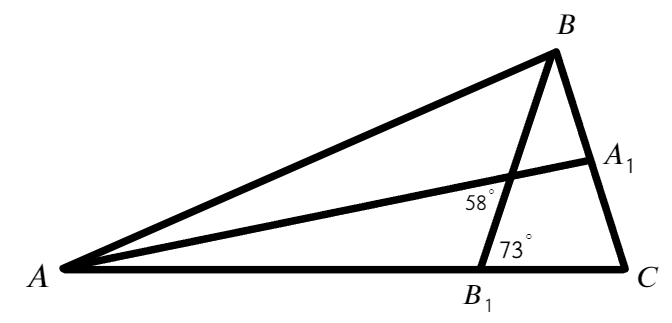
\includegraphics[scale=0.35]{g1072.png}}
\end{figure}\\
Найдём $\angle A_1AC=180^\circ-58^\circ-(180^\circ-73^\circ)=15^\circ,$ значит $\angle A=2\cdot15^\circ=30^\circ.$ Тогда $\angle ABB_1=180^\circ-30^\circ-107^\circ=43^\circ,\ \angle B=2\cdot43^\circ=86^\circ,\ \angle C=180^\circ-30^\circ-86^\circ=64^\circ.$\\
